\documentclass[a4paper]{report}

%% Language and font encodings
\usepackage[english,russian]{babel}
\usepackage[utf8x]{inputenc}
%\usepackage[cp1251]{inputenc}
\usepackage[T1]{fontenc}
\usepackage{caption}
\usepackage{subcaption}
%% Sets page size and margins
\usepackage[a4paper,top=3cm,bottom=2cm,left=3cm,right=3cm,marginparwidth=1.75cm]{geometry}

%% Useful packages
\usepackage{amsmath}
\usepackage{graphicx}
\usepackage[colorinlistoftodos]{todonotes}
\usepackage[colorlinks=true, allcolors=blue]{hyperref}

\setcounter{secnumdepth}{0}

\title{Лабораторная работа: нанопроволки}
\author{Евгений Сафронов}
\date{Осенний семестр, 4 курс}

\begin{document}
\maketitle


\section{Осаждение никеля на подложку}

В ходе лабораторной работы сначала было выполнено осаждение без мембраны с порами для нанопроволок.

\begin{figure}[h]
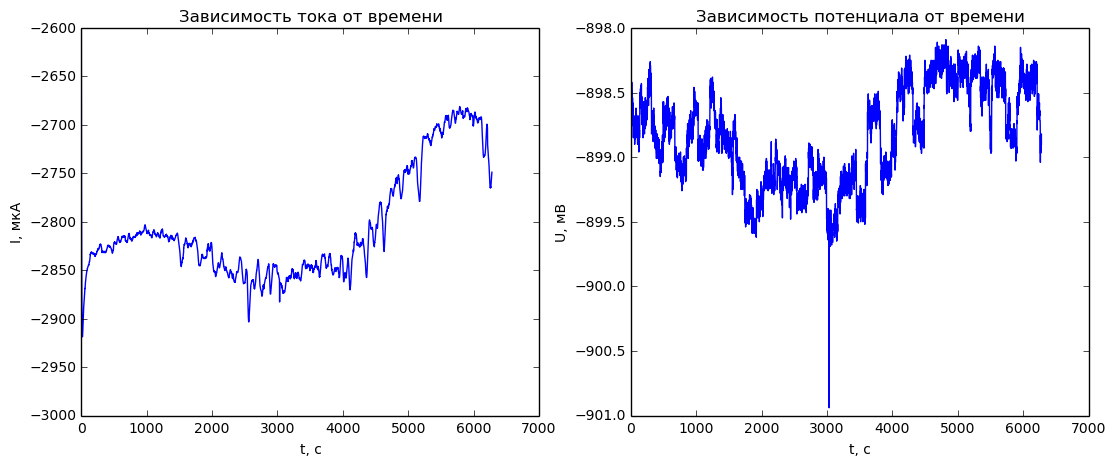
\includegraphics[width=1\textwidth]{nomem.png}
\caption{\label{fig:nomem}Процесс осаждения без мембраны}
\end{figure} 

Выход по току составил $95\%$
\newline
\newline
А потом и через мембрану

\begin{figure}[h]
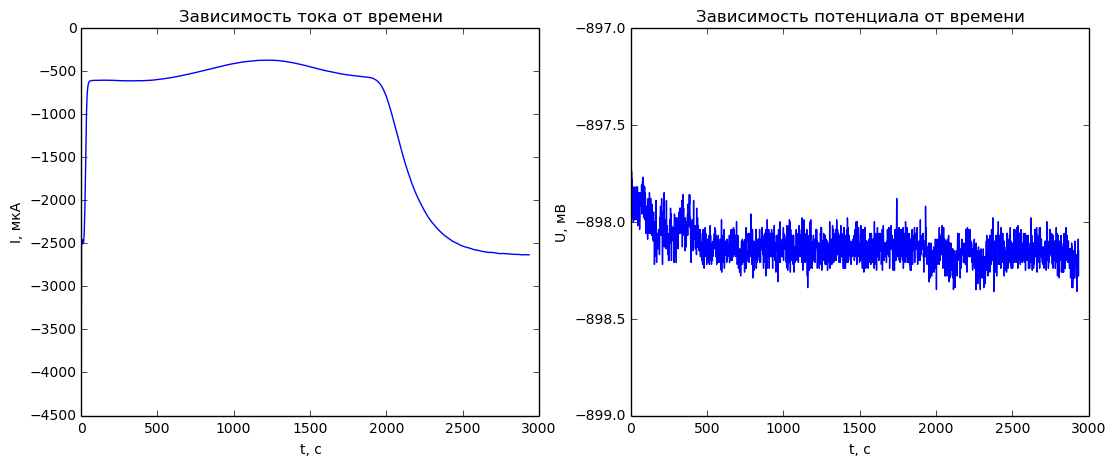
\includegraphics[width=1\textwidth]{mem.png}
\caption{\label{fig:mem}Процесс осаждения через мембрану}
\end{figure}

\end{document}